\chapter{\bf{Activity Diagrams}}

\section{Apertura e Chiusura Cancello [Scenario 1]}
Questo scenario, illustrato in figura \ref{scenario1}, descrive in sequenza le azioni che l’utente compie per aprire e chiudere il cancello, dalle fasi iniziali di richiesta tramite il pulsante B1, fino al feedback visivo che conferma l'operazione completata.
Di seguito vengono presentati i flussi di azioni associati allo scenario corrente. \\

\noindent Apertura del Cancello:
\begin{enumerate}
    \item L’utente decide di aprire il cancello e si avvicina ad esso;
    \item Per avviare il processo di apertura, l’utente preme il pulsante B1;
    \item Il sistema rileva che il pulsante B1 è stato premuto;
    \item Il sistema verifica che il cancello sia chiuso o in chiusura;
    \item Il sistema avvia il processo di apertura del cancello;
    \item Durante l'apertura, il dispositivo fornisce un feedback visivo attivando il lampeggiamento del LED giallo con frequenza 0.5 Hz;
    \item Una volta completata l'apertura, tutti i LED (giallo, rosso e verde) si accendono staticamente per indicare la completa apertura del cancello.
\end{enumerate}

\noindent \\ Chiusura del Cancello:
\begin{enumerate}
    \item L’utente decide di chiudere il cancello e si avvicina ad esso;
    \item Per avviare il processo di chiusura, l’utente preme il pulsante B1;
    \item Il sistema rileva che il pulsante B1 è stato premuto;
    \item Il sistema verifica che il cancello sia aperto o in apertura;
    \item Il sistema avvia il processo di chiusura del cancello;
    \item Durante la chiusura, il dispositivo fornisce un feedback visivo attivando il lampeggiamento del LED giallo con frequenza 0.5 Hz;
    \item Una volta completata la chiusura, tutti i LED (giallo, rosso e verde) si spengono per indicare la completa chiusura del cancello.
\end{enumerate}

\begin{figure}[H]
    \centering
    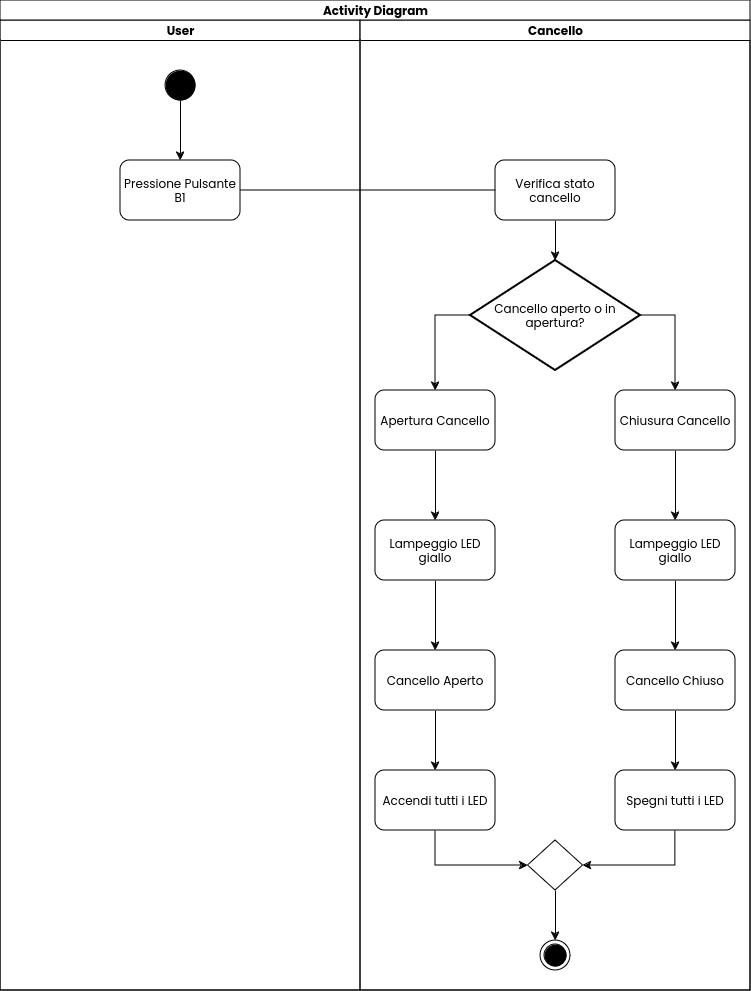
\includegraphics[width=0.9\textwidth]{figures/scenario1.png}
    \caption{Scenario 1}
    \label{scenario1}
\end{figure}


\section{Regolazioni [Scenario 2]}
\noindent Questo scenario è suddiviso in due parti, entrambe ricostruite in figura \ref{scenario2}, poiché i diagrammi di entrambe le parti sono identici sotto il profilo funzionale, è stato preferito l'inserimento di un singolo diagramma esemplificativo per entrambi.\\

La prima parte dello scenario descrive sequenzialmente le azioni che l’utente compie per regolare il tempo di chiusura automatica del cancello.
Di seguito viene presentato il flusso di azioni associato alla sezione corrente. \\

\noindent Regolazione Tempo di Chiusura Automatica:

\begin{enumerate}
    \item L’utente decide di regolare il tempo di chiusura automatica del cancello;
    \item L’utente si avvicina al cancello chiuso;
    \item Per avviare il processo di regolazione, l’utente preme il pulsante B2;
    \item Il sistema rileva che il pulsante B2 è stato premuto;
    \item Il tempo di chiusura automatica viene così gestito:
    
    \begin{enumerate}
        \item Se il tempo di chiusura automatica è inferiore a 120 secondi, ogni pressione del pulsante B2 aumenta il tempo di 10 secondi;
        \item Se il tempo di chiusura automatica è già a 120 secondi, premendo nuovamente B2 il tempo viene riportato a 10 secondi. \\
    \end{enumerate}
\end{enumerate}

La seconda parte descrive, invece, le azioni che l’utente compie per regolare la durata delle fasi di apertura e chiusura del cancello. \\

\noindent Regolazione Tempo di Lavoro:

\begin{enumerate}
    \item L’utente decide di regolare la durata delle fasi di apertura e chiusura del cancello;
    \item L’utente si avvicina al cancello chiuso;
    \item Per avviare il processo di regolazione, l’utente preme il pulsante B3;
    \item Il sistema rileva che il pulsante B3 è stato premuto;
    \item Il tempo per la regolazione delle fasi viene così gestito:
    \begin{enumerate}
        \item Se il tempo di chiusura automatica è inferiore a 120 secondi, ogni pressione del pulsante B3 aumenta il tempo di 10 secondi;
        \item Se il tempo di chiusura automatica è già a 120 secondi, premendo nuovamente B3 il tempo viene riportato a 10 secondi. \\
    \end{enumerate}
\end{enumerate}

\begin{figure}[H]
    \centering
    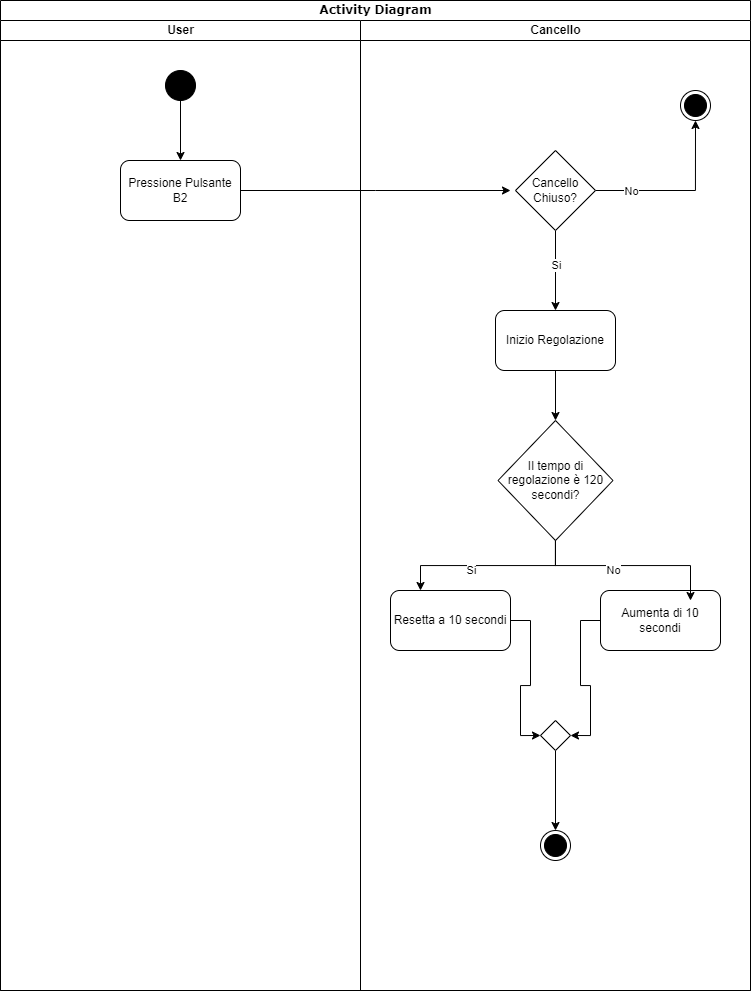
\includegraphics[width=0.9\textwidth]{figures/scenario2.png}
    \caption{Scenario 2}
    \label{scenario2}
\end{figure}


\section{Gestione Stato e Ostacoli [Scenario 3]}
\noindent Lo scenario attuale, ritratto in figura \ref{scenario3}, è anch'esso suddiviso in due sezioni differenti. \\

La prima parte descrive in modo consecutivo le azioni relative alla riapertura automatica del cancello, attuata dal dispositivo, in presenza di un ostacolo.
Di seguito è presentato il flusso di azioni associato allo scenario corrente. \\

\noindent Riapertura Automatica con Rilevazione Ostacolo:

\begin{enumerate}
    \item Il sistema rileva un ostacolo tramite il sensore di presenza (P1) durante la fase di chiusura del cancello;
    \item Il sistema avvia la riapertura automatica del cancello per evitare danni e garantire la sicurezza;
    \item Il dispositivo fornisce un feedback visivo in caso di apertura completa del cancello, accendendo tutti i LED (giallo, rosso e verde);
    \item Se il sistema non rileva alcun ostacolo procederà con la chiusura del cancello e l'attivazione del sensore di presenza P2.
\end{enumerate}

La seconda parte descrive, invece, le azioni compiute dal sistema per gestire l'apertura o la chiusura del cancello in presenza di ostacoli.
Di seguito viene presentato il flusso di azioni associato allo scenario corrente. \\

\noindent Gestione Richieste in Presenza di Ostacoli:

\begin{enumerate}
    \item Il sistema rileva la presenza di un ostacolo tramite il sensore P1;
    
    \item Il sistema ignora le richieste di apertura o chiusura del cancello per prevenire movimenti non sicuri;
    
    \item Il dispositivo fornisce un feedback visivo della presenza di un ostacolo, facendo lampeggiare il LED verde con una frequenza di 1 Hz per un massimo di 30 secondi o finché l'ostacolo non viene più rilevato.
\end{enumerate}

\begin{figure}[H]
    \centering
    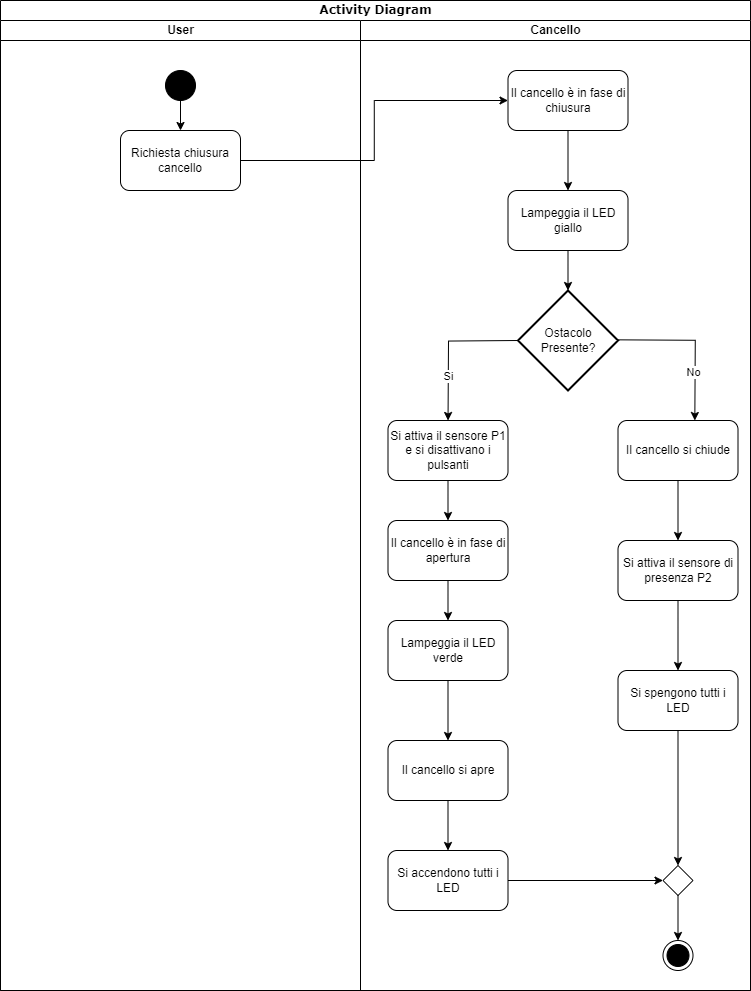
\includegraphics[width=0.9\textwidth]{figures/scenario3.png}
    \caption{Scenario 3}
    \label{scenario3}
\end{figure}


\section{Stato di Errore [Scenario 4]}
Questo scenario, riprodotto in figura \ref{scenario4}, descrive in modo seriale le azioni che portano il dispositivo in uno stato di errore.
Di seguito viene presentato il flusso di azioni associato allo scenario corrente. \\

\noindent Stato di Errore con Rilevazione Malfunzionamento del Sensore:

\begin{enumerate}
    \item L’utente richiede la chiusura del cancello tramite il pulsante B1;
    
    \item Il sistema rileva che il sensore di presenza (P2) non si è attivato dopo il tempo di lavoro previsto durante la fase di chiusura del cancello;
    
    \item Il sistema entra in uno stato di errore per avvisare l’utente;
    
    \item Il dispositivo fornisce un feedback visivo dello stato di errore accendendo il LED rosso se il cancello non si chiude entro 10 secondi dalla scadenza del tempo di lavoro.
\end{enumerate}

\begin{figure}[H]
    \centering
    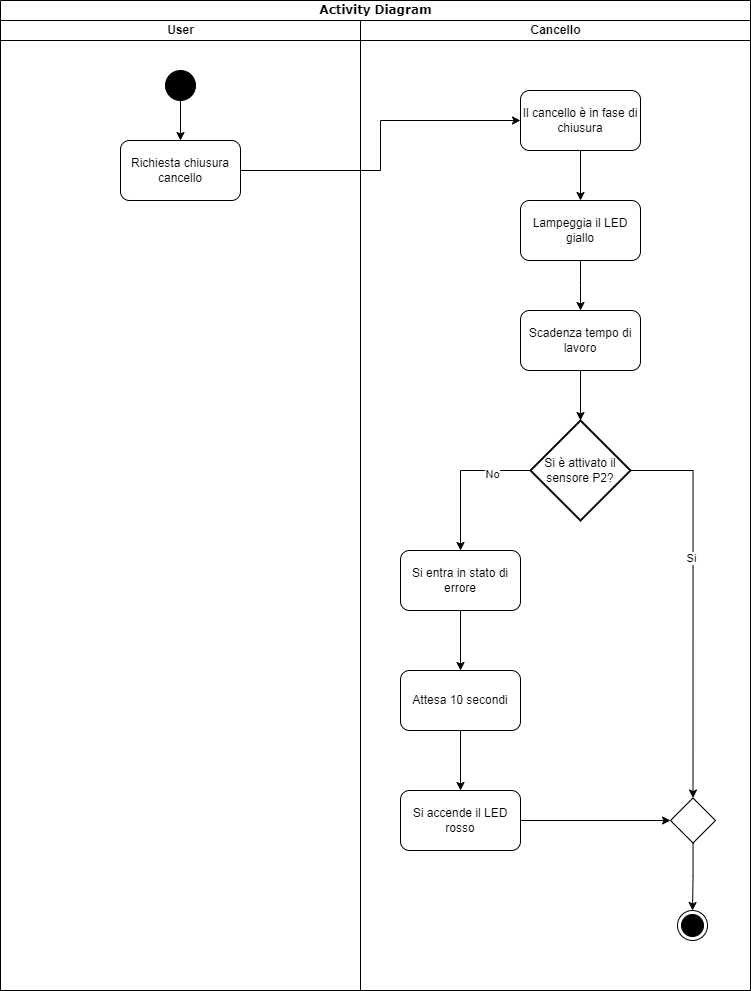
\includegraphics[width=0.9\textwidth]{figures/scenario4.png}
    \caption{Scenario 4}
    \label{scenario4}
\end{figure}


\section{Chiusura Automatica all'accensione [Scenario 5]}
Questo scenario, rappresentato in figura \ref{scenario5}, descrive in successione le azioni necessarie per la chiusura automatica del cancello all'accensione del dispositivo.
Nell'elenco sottostante è presentato il flusso di azioni associato allo scenario corrente. \\

\noindent Chiusura Automatica all'Accensione del Dispositivo:

\begin{enumerate}
    \item L’utente accende il dispositivo per la prima volta;
    \item Il sistema verifica che i sensori di presenza P1 e P2 non siano attivi;
    \item Il sistema avvia la procedura di chiusura del cancello;
    \item Il dispositivo garantisce la corretta chiusura del cancello all'accensione.
\end{enumerate}

\begin{figure}[H]
    \centering
    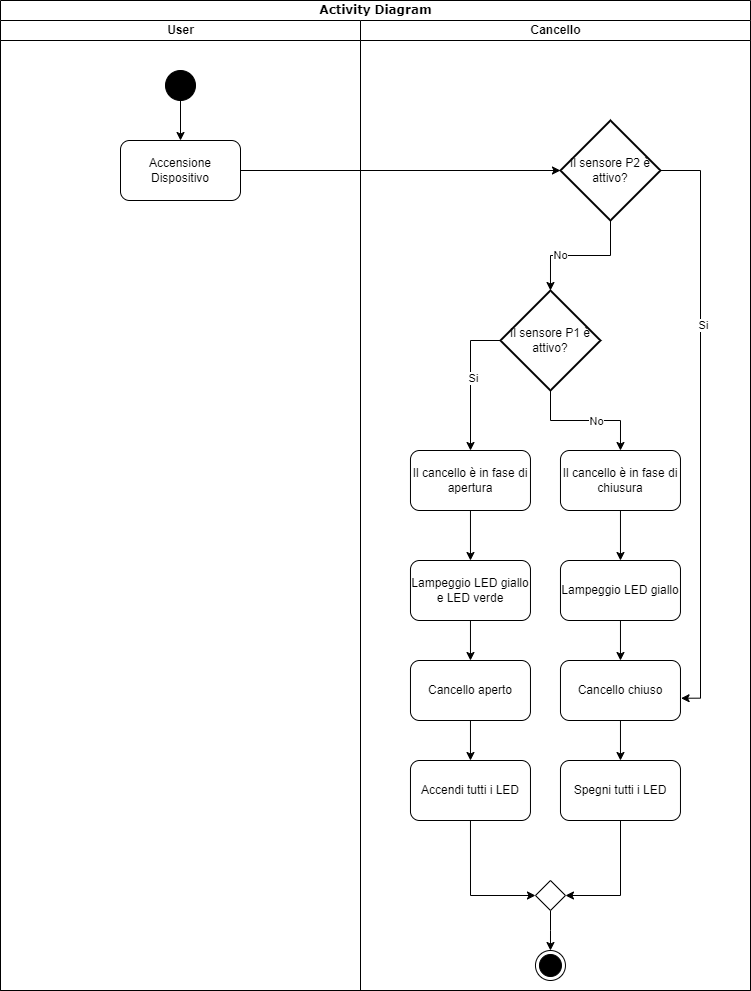
\includegraphics[width=0.9\textwidth]{figures/scenario5.png}
    \caption{Scenario 5}
    \label{scenario5}
\end{figure}